%%%%%%%%%%%%%%%%%%%%%%%%%%%%%%%%%%%%%%%%%
% Beamer Presentation
% LaTeX Template
% Version 1.0 (10/11/12)
%
% This template has been downloaded from:
% http://www.LaTeXTemplates.com
%
% License:
% CC BY-NC-SA 3.0 (http://creativecommons.org/licenses/by-nc-sa/3.0/)
%
%%%%%%%%%%%%%%%%%%%%%%%%%%%%%%%%%%%%%%%%%

%----------------------------------------------------------------------------------------
%	PACKAGES AND THEMES
%----------------------------------------------------------------------------------------

\documentclass{beamer}

\mode<presentation> {

% The Beamer class comes with a number of default slide themes
% which change the colors and layouts of slides. Below this is a list
% of all the themes, uncomment each in turn to see what they look like.

%\usetheme{default}
%\usetheme{AnnArbor}
%\usetheme{Antibes}
%\usetheme{Bergen}
%\usetheme{Berkeley}
%\usetheme{Berlin}
%\usetheme{Boadilla}
%\usetheme{CambridgeUS}
%\usetheme{Copenhagen}
%\usetheme{Darmstadt}
%\usetheme{Dresden}
%\usetheme{Frankfurt}
%\usetheme{Goettingen}
%\usetheme{Hannover}
%\usetheme{Ilmenau}
%\usetheme{JuanLesPins}
%\usetheme{Luebeck}
\usetheme{Madrid}
%\usetheme{Malmoe}
%\usetheme{Marburg}
%\usetheme{Montpellier}
%\usetheme{PaloAlto}
%\usetheme{Pittsburgh}
%\usetheme{Rochester}
%\usetheme{Singapore}
%\usetheme{Szeged}
%\usetheme{Warsaw}

% As well as themes, the Beamer class has a number of color themes
% for any slide theme. Uncomment each of these in turn to see how it
% changes the colors of your current slide theme.

%\usecolortheme{albatross}
%\usecolortheme{beaver}
%\usecolortheme{beetle}
%\usecolortheme{crane}
%\usecolortheme{dolphin}
%\usecolortheme{dove}
%\usecolortheme{fly}
%\usecolortheme{lily}
%\usecolortheme{orchid}
%\usecolortheme{rose}
%\usecolortheme{seagull}
%\usecolortheme{seahorse}
%\usecolortheme{whale}
%\usecolortheme{wolverine}

%\setbeamertemplate{footline} % To remove the footer line in all slides uncomment this line
%\setbeamertemplate{footline}[page number] % To replace the footer line in all slides with a simple slide count uncomment this line

%\setbeamertemplate{navigation symbols}{} % To remove the navigation symbols from the bottom of all slides uncomment this line
}

\usepackage{graphicx} % Allows including images
\usepackage{booktabs} % Allows the use of \toprule, \midrule and \bottomrule in tables
\usepackage{listings}
\usepackage{amsmath}
\usepackage{algpseudocode,algorithm,algorithmicx}

\lstdefinestyle{customjava}{
  breaklines=true,
  frame=L,
  xleftmargin=\parindent,
  language=Java,
  showstringspaces=false,
  basicstyle=\footnotesize\ttfamily,
  keywordstyle=\bfseries\color{green!40!black},
  commentstyle=\itshape\color{gray!40!black},
  identifierstyle=\color{blue},
  stringstyle=\color{orange},
}

%----------------------------------------------------------------------------------------
%	TITLE PAGE
%----------------------------------------------------------------------------------------

\title[Data link layer]{Data link layer} % The short title appears at the bottom of every slide, the full title is only on the title page

\author{Jonathan Windle} % Your name
\institute[UEA] % Your institution as it will appear on the bottom of every slide, may be shorthand to save space
{
University of East Anglia \\ % Your institution for the title page
\medskip
\textit{J.Windle@uea.ac.uk} % Your email address
}
\date{\today} % Date, can be changed to a custom date

\begin{document}

\begin{frame}
\titlepage % Print the title page as the first slide
\end{frame}

\begin{frame}[allowframebreaks]
\frametitle{Overview} % Table of contents slide, comment this block out to remove it
\tableofcontents % Throughout your presentation, if you choose to use \section{} and \subsection{} commands, these will automatically be printed on this slide as an overview of your presentation
\end{frame}

%-----------------------------------------------------------------
\section{Intro}
\begin{frame}
\frametitle{Intro}
\begin{itemize}
\item Main task of data link layer is to take the raw transmission facility, via the physical layer, and transform it into a connection which is free from errors.
\item Achieves this by employing error detection and error correction onto the sequence of transmitted data.
\item Error detection is used to request re-transmission of corrupt packets.
\item Error correction attempts to correct errors without the need for re-transmission.
\item Data link layer is also concerned with creating frames from network layer packets.
\item Concerned with traffic regulation, to stop fast sender swamping slower receiver.
\item Controls data flow on bi-directional channels.
\end{itemize}
\end{frame}
%----------------------------------------------------------------
\section{Backwards Error Correction}
\begin{frame}
\frametitle{Backwards Error Correction}
\begin{itemize}
\item Is a two stage process:
\begin{itemize}
\item Error detection
\item Retransmission for correction.
\end{itemize}
\item Common techniques used:
\begin{itemize}
\item Character Parity Bits
\item Longitudinal Parity Bits
\item Cyclic Redundancy Checks
\end{itemize}
\end{itemize}
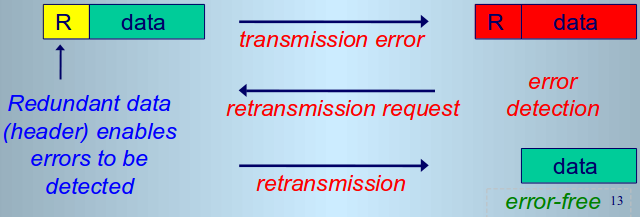
\includegraphics[scale=0.3]{bec.png}
\end{frame}
%------------------------------------------------------------------
\subsection{Character Parity Bits}
\begin{frame}
\frametitle{Character Parity Bits}
\begin{itemize}
\item Utilises an additional bit which is computed and attached to eaach character.
\item Either odd parity or even parity.
\item Adding parity bit detects errors which affect an odd number of bits. Unfortunately errors typically occur in bursts.
\end{itemize}
\end{frame}
%---------------------------------------------------------------
\subsection{Longitudinal Parity Bits}
\begin{frame}
\frametitle{Longitudinal Parity Bits}
\begin{itemize}
\item Technique also calleda Block Check Sum (BCS).
\item A collection of octetes (each using odd/even parity) is treated as a block.
\item Bits in position 1 of each octet are checked by a parity bit. Similarly for bits in position 2 checked by parity bit and so on.
\item Can detect all 2 and 3 bit errors within the block, but miss some patterns involving 4 bits.
\end{itemize}
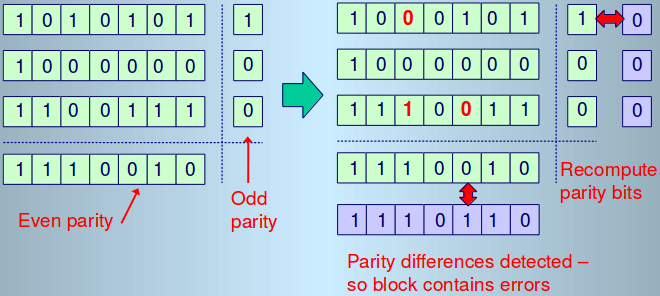
\includegraphics[scale=0.3]{lpb.png}
\end{frame}
%------------------------------------------------------------------
\subsection{Cyclic Redundancy Check}
\begin{frame}
\frametitle{Cyclic Redundancy Check}
\begin{itemize}
\tiny
\item The basic principle is that the transmitter treats the message as a binary number and divides the data by a pre-defined constant to give a remainder.
\item Remainder is then subtracted from the data and this is then transmitted to the receiver.
\item The receiver performs the same division which should result in no remainder.
\item If the division does result in a non-zero remainder then the data has been corrupted.
\item Polynomial Generators:
\begin{itemize}
\tiny
\item Bit strings are treated as polynomials with coefficientss of 0 and 1 i.e.\\
$11001 = x^4+x^3+x^0$
\item An $n$ bit polynomial generator produces an $n-1$ bit remainder.
\end{itemize}
\item A 16 bit CRC will identify:
\begin{itemize}
\tiny
\item All single and double errors
\item All odd numbers of bit corruptions
\item All bursts of errors of length $\leq$ 16
\item 99.997\% of 17 bit burst errors and 99.998\% of 18 bit burst errors.
\end{itemize}
\end{itemize}
\end{frame}
%------------------------------------------------------------------
\section{Forward Error Correction}
\begin{frame}
\frametitle{Forward Error Correction}
\begin{itemize}
\item On unidirectional connections it is not possible to send any feedback from the receiver to the transmitter.
\item Makes it impossible to detect errors and ask for retransmission.
\item Instead provide sufficient redundant information to enable error correction at receiver.
\item Techniques rely on encoding additional redundancy into the data to allow for error correction.
\item FEC also important for real-time communication where insufficient time to request retransmission and await new data.
\item For any data encoding scheme, the {\color{red}Hamming Distance} is the number of bits which differ between valid codes.
\item Can use XOR operator to determine the Hamming Distance. 
\item If two codewords are Hamming Distance $d$ bits apart, then it will require $d$ single bit errors to convert one into another.
\end{itemize}
\end{frame}
%------------------------------------------------------------------
\subsection{Hamming Codes}
\begin{frame}
\frametitle{Hamming Codes}
\begin{itemize}
\item Categorised by the number of data bits and parity bits which form the transmitted codeword.
\item For example a (7,4) Hamming Code comprises of 7 bits encoding, 4 bits data, hence 3 parity bits.
\item More parity bits, gives more chance of detecting bit errors.
\item For effective forward error correction a proportion of 50\% data 50\% parity is necessary.
\item This reduces the effective data rate by a factor of 2.
\item FEC can be usedon bi-directional channels, butis inefficient for all but the most unreliable channels.
\end{itemize}
\end{frame}
%-----------------------------------------------------------------
\subsubsection{Simple Hamming Code}
\begin{frame}
\frametitle{Simple Hamming Code}
Creation:
\begin{itemize}
\item Bits that are a power of 2 are parity bits. The rest are data bits.
\item Determine which data bits are used in each parity bit by using addition.
\item For a 7,4 code:
\begin{itemize}
\item P0 = parity(D0,D1,D3)
\item P1 = parity(D0,D2,D3)
\item P2 = parity(D1,D2,D3)
\end{itemize}
\end{itemize}
Correction:
\begin{itemize}
\item When arrives, the parities are calculated again using the data bits.
\item There are then compared to the received parity bits, where K=0:
\begin{itemize}
\item P0 $\neq$ P0' ; error: K=K+1
\item P1 $\neq$ P1' ; error: K=K+2
\item P2 $\neq$ P2' ; error: K=K+4
\end{itemize}
\item If K = 0, codeword is accepted.
\item Otherwise K points to the erronous bit in codeword
\end{itemize}
\end{frame}
%-----------------------------------------------------------------
\begin{frame} 
\Huge{\centerline{The End}}
\end{frame}
\end{document}